\documentclass[10pt,a4paper]{article}
\usepackage[T1]{fontenc}
\usepackage[utf8]{inputenc}
\usepackage{lmodern}
\usepackage[margin=2.2cm]{geometry}
\usepackage{microtype}
\usepackage{booktabs}
\usepackage{longtable}
\usepackage{tabularx}
\usepackage{array}
\usepackage{graphicx}
\usepackage{xcolor}
\usepackage{pifont}
\usepackage{enumitem}
\usepackage{tikz}
\usetikzlibrary{arrows.meta,positioning}
\usepackage[hidelinks]{hyperref}

\definecolor{harbor}{RGB}{14,124,134}
\newcommand{\cmark}{\textcolor{harbor}{\ding{51}}}
\newcommand{\xmark}{\textcolor{red!70!black}{\ding{55}}}
\setlist{itemsep=2pt,topsep=4pt}
\setlength{\emergencystretch}{2em}
% Generated table rows (report/tables.ts); the primitive input works inside tabular before \bottomrule.
\makeatletter\newcommand{\rows}[1]{\@@input #1 }\makeatother

\title{\textbf{Harbor}\\[2pt]\large Personal layouts for websites you never set up,\\ with Meta Muse Spark~1.3 and SAM~3.1\\[2pt]\normalsize Technical report}
\author{Tymon Żarski}
\date{Meta AI Developer Hackathon --- status at 4 November 2026 (submission)}

\begin{document}
\maketitle

\begin{abstract}
\noindent Harbor is a Chrome extension that reads a web page the user has never configured, asks Meta's Muse Spark~1.3 for a bounded layout plan, previews the plan on the real page and applies it reversibly. With the user's consent it learns which items they open and suggests emphasising them; the page changes only when they accept. The user can state what they come to the page for (``I only read the feed: hide both sidebars''); the plan hides, compacts, lays out as a grid, or emphasises regions of the site's own markup, never rewriting it. A screenshot can optionally be segmented with SAM~3.1 to give the planner visual groups. We built an evaluation set of 54 scenarios on 20 popular live websites with 124 checkable expectations, including 52 ``keep'' checks that catch over-hiding, and a runner that drives the extension through each scenario and checks the outcome on the live page. Three evaluation rounds found and fixed two real defects; in the last round the extension met 93\% of expectations and fully completed 84\% of scenarios, with no over-hiding, against 42\% and 0\% for leaving the page unchanged. Sending the screenshot to SAM made no consistent difference on this set. A round costs about \$2.25 of Spark tokens at listed prices. Since those rounds (28--29 October) we added a three-pick onboarding whose choices go with every request as rules the user's choice overrides, region-level fingerprints that re-find saved layouts after a page changes (96.2\% correct and 0.9\% wrong on held-out synthetic page changes, against 82.4\% and 1.9\% for the previous matcher), kept layouts that come back by themselves, site-wide header changes, and a learned item order for rows of like items (\S\ref{sec:since}). These were tested on owned test pages and offline snapshots; the live-site rounds were not re-run on them.
\end{abstract}

\section{Problem}
People use a handful of crowded websites every day --- a code host, a Q\&A site, a video site, a shop --- and each serves the same distractions on every visit: marketing navigation, sign-up bars, recommendation columns, action buttons they never press. Fixing this today means writing CSS selectors in a user-style extension, which few people can do and which breaks when the site changes its markup. Reader modes help only on articles.

Harbor\footnote{Planned and first built under the working name ``Smart Web''; renamed on 29 October 2026. Internal identifiers keep the old name: the repository and package names and the \texttt{data-smart-web-*} attributes the extension sets on pages.} lets a person say, in their own words, what they come to a page for, and turns that into a reviewed, reversible change to the page itself. The request that shaped the project came from the author's own use of GitHub, verbatim: \emph{``please hide completly. i do not use at all the actions [unpin,watch,fork,start] neither on the top bar neitiher in the sidebar''}. It names the same controls in two places, which a single selector would miss.

\paragraph{Contributions.}
\begin{itemize}
\item An MV3 extension that scans a page, obtains a validated Meta layout plan, previews it, applies it, restores the page, follows the tab across navigation, re-applies the layout when a single-page app redraws a region, and reuses saved plans on later visits and on other pages of the same kind without a model call (\S\ref{sec:system}).
\item Learning from use: opt-in, on-device counts of what the user opens, turned into suggestions that change the page only when accepted (\S\ref{sec:system}).
\item A planner contract: strict JSON schema, a local validator with one repair round, user goals, and follow-up questions whose answers adjust the plan locally (\S\ref{sec:meta}).
\item An evaluation set of real sites and requests with machine-checkable expectations, a runner that measures outcomes on the live page, and three scored rounds (\S\ref{sec:eval}, \S\ref{sec:results}).
\item Added after the rounds: a user profile sent as named rules, with every change traced to its rule; region-level fingerprints for saved layouts with an offline held-out benchmark; and a learned order for rows of like items applied without moving the DOM (\S\ref{sec:since}).
\end{itemize}

\section{System}\label{sec:system}

\begin{figure}[t]
\centering
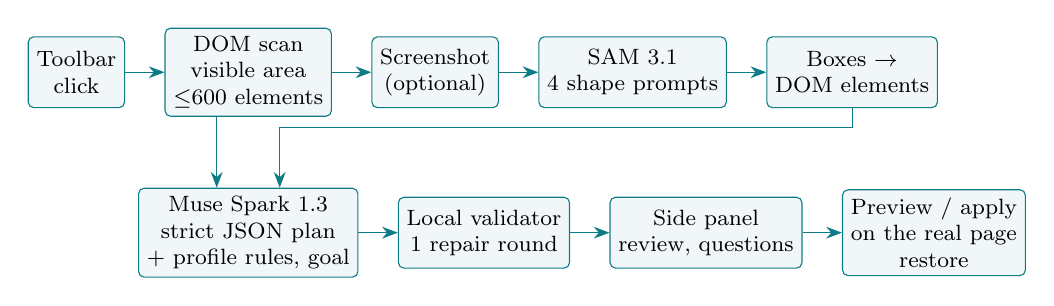
\begin{tikzpicture}[node distance=4mm and 5mm, box/.style={draw=harbor, rounded corners=2pt, fill=harbor!6, align=center, font=\footnotesize, minimum height=9mm, inner sep=3pt}, arr/.style={-{Stealth[length=2mm]}, harbor}]
\node[box] (click) {Toolbar\\click};
\node[box, right=of click] (scan) {DOM scan\\visible area\\$\le$600 elements};
\node[box, right=of scan] (shot) {Screenshot\\(optional)};
\node[box, right=of shot] (sam) {SAM 3.1\\4 shape prompts};
\node[box, right=of sam] (hit) {Boxes $\rightarrow$\\DOM elements};
\node[box, below=9mm of scan] (spark) {Muse Spark 1.3\\strict JSON plan\\+ profile rules, goal};
\node[box, right=of spark] (val) {Local validator\\1 repair round};
\node[box, right=of val] (panel) {Side panel\\review, questions};
\node[box, right=of panel] (page) {Preview / apply\\on the real page\\restore};
\draw[arr] (click) -- (scan);
\draw[arr] (scan) -- (shot);
\draw[arr] (shot) -- (sam);
\draw[arr] (sam) -- (hit);
\draw[arr] ([xshift=-4mm]scan.south) -- ([xshift=-4mm]spark.north);
\draw[arr] (hit.south) -- ++(0,-2.5mm) -| ([xshift=4mm]spark.north);
\draw[arr] (spark) -- (val);
\draw[arr] (val) -- (panel);
\draw[arr] (panel) -- (page);
\end{tikzpicture}
\caption{Pipeline. Meta calls go through a local LiteLLM proxy that holds the API key and a spend cap; the extension never sees the provider key.}
\label{fig:pipeline}
\end{figure}

\paragraph{Scan.} On a toolbar click the extension injects a content script (Chrome's \texttt{activeTab}; no standing access to sites) that records the visible elements: tag, role, a coarse kind (landmark, interactive, list, item, heading, media, group), parent, bounding box, up to 80 characters of visible text, link path and a few identifying attributes. Visibility uses \texttt{checkVisibility}, so closed menus and faded elements are left out. Form fields are listed without their contents and can never be targeted. Each element gets an ID valid only for this scan; the page refuses IDs from an older scan, so a plan can never mark the wrong element after the site re-renders.

\paragraph{Plan.} Spark receives one line per element (\texttt{id <tag> kind parent=id [x,y,w,h] attrs href "text"}), the URL, the user's goal if given, and optionally SAM's visual groups. It returns, under a strict JSON schema, groups (a container, its members, a role and a reason), one operation per group from \texttt{hide-secondary}, \texttt{collapse} (shown as Fold, added 2 November), \texttt{compact}, \texttt{grid}, \texttt{emphasize}, \texttt{none}, a URL pattern per group (site chrome gets a broad pattern, view-specific content a narrow one), and one to three follow-up questions whose options name the plan changes they imply. Answers are applied locally, without another call.

\paragraph{Validate and repair.} A local validator rejects unknown or stale IDs, form fields, members outside their container, members claimed by two groups, grids of fewer than two items, oversized plans, URL patterns that do not match the page, and reorderable groups without a stable identity. If anything is rejected, Spark gets one repair round with the validator's messages; whatever still fails is dropped.

\paragraph{Apply and restore.} The executor never moves or rewrites the site's DOM. It sets data attributes on the site's own elements and inserts one stylesheet keyed on them; restore removes both. Preview shows hidden regions dimmed and outlined in place, and Escape on the page undoes it. Links, focus order and the site's scripts keep working. A hide takes the plan's whole region only when the named members are most of it; otherwise only the members are hidden (\S\ref{sec:results}).

\paragraph{Remember and follow.} An applied plan is saved per page with node signatures; on the next visit, or on another page matching a group's URL pattern (e.g.\ \texttt{github.com/\{owner\}/\{repo\}/*}), it is remapped to the new scan and re-applied with no model call. Lists are re-found by row shape only when the plan covered the whole list. With the user's permission for a site, the extension follows the tab across navigation. ``Hide something else'' lets the user point at any element, widen or narrow the selection, and hide it; such hides are saved with the plan and survive a new plan.

\paragraph{Redraws.} Single-page apps such as YouTube and GitHub replace whole regions when they re-render, which drops the marks. While a layout is kept, the page watches for marked elements leaving the document; once the burst settles the extension reads the page again and the saved plan re-applies, with no model call. A page that redraws more than five times in 30 seconds gets a notice instead, so a site that reacts to the change itself cannot loop.

\paragraph{Learning from use.} Off until the user turns it on for a site. While a layout is kept, real clicks (\texttt{isTrusted}; scripted clicks are ignored) on items of its groups, including groups the plan leaves unchanged, are learned on the device by the author's pre-event ranker: a decaying per-item count blended with a small network on the press's pointer features (press length, approach speed, hover time and similar; no content is recorded). When one item has at least three uses and holds most of its group's weight, the panel asks: \emph{``You opened `Summit 45' 3 times. Highlight it in Backpack cards?''} Accepting adds a learned \texttt{emphasize} group over the plan, saved with it so it returns on later visits; either answer is remembered and the suggestion is not repeated; Reset clears what was learned, model included. Until 2 November learned changes were limited to emphasis; the learned order of \S\ref{sec:since} now also reorders, visually only, with the trade-off stated there.

\begin{figure}[t]
\centering
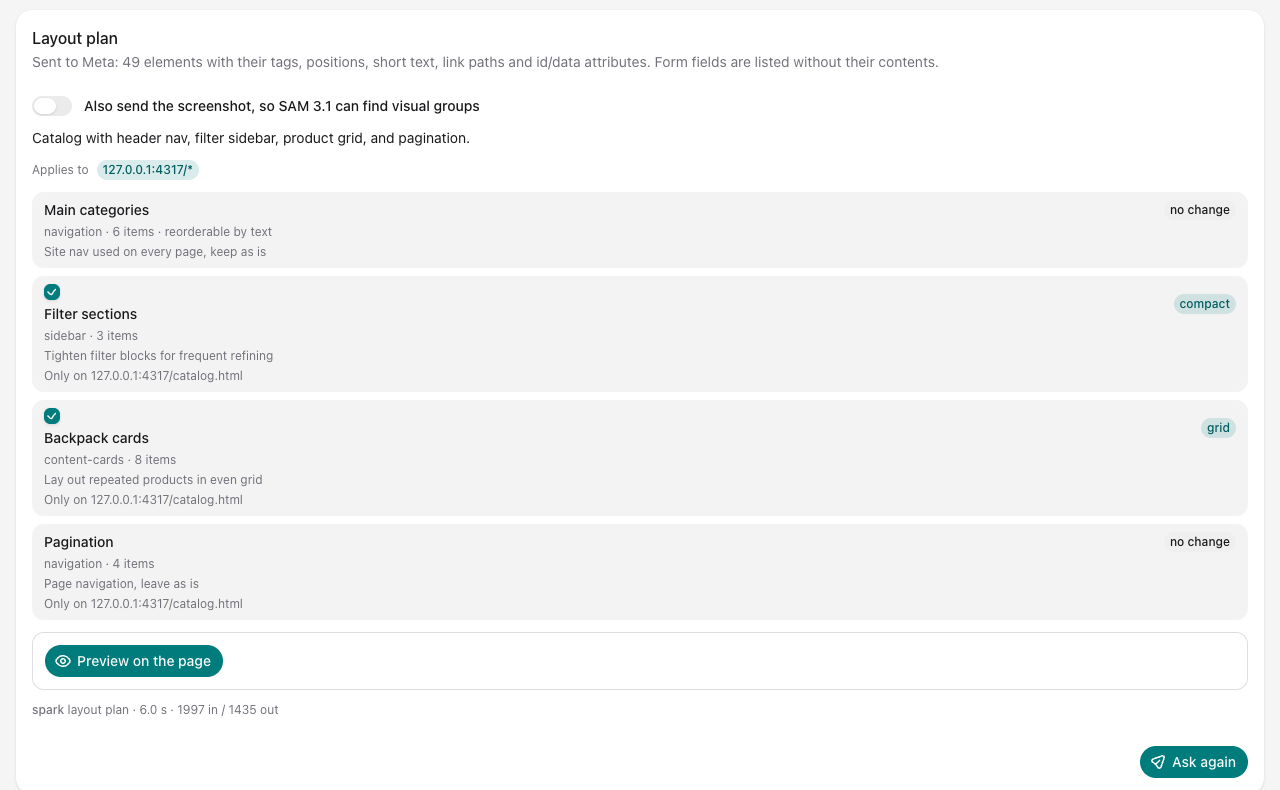
\includegraphics[width=0.49\linewidth]{figures/panel-plan.png}\hfill
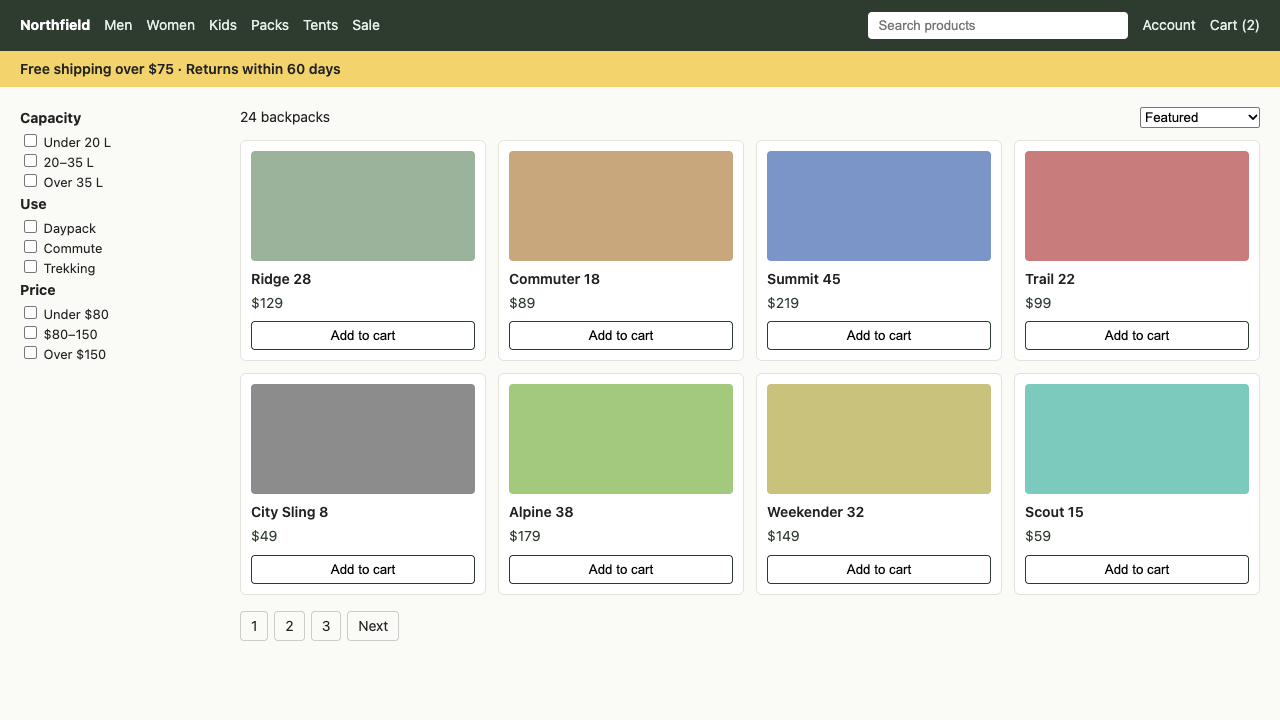
\includegraphics[width=0.49\linewidth]{figures/catalog-applied.png}
\caption{Owned test page. Left: the side panel with a live Spark plan (6.0\,s): filters \texttt{compact}, product cards \texttt{grid}, navigation and pagination left alone, each with its reason and URL scope. Right: the same page after Keep; the cards were five and three per row before.}
\label{fig:fixture}
\end{figure}

\section{Use of Meta models}\label{sec:meta}
\paragraph{Muse Spark 1.3} does the planning: it reads an arbitrary page structure, names its regions, maps the user's goal onto them (including the same thing appearing in two places), chooses operations, writes URL patterns that generalise across pages of the same kind, and asks questions. Strict \texttt{json\_schema} output held on every call, directly and through LiteLLM. Reasoning is about 70--90\% of output tokens; \texttt{reasoning\_effort: low} halved latency on our fixtures with the same plans and is the default. The first prompt produced ``no change'' for regions its own reasons called low-value; stating what a useful plan changes, and taking the user's goal, fixed this.

\paragraph{SAM 3.1} finds visually similar regions in the screenshot. Probing on UI screenshots showed it responds to shape phrases (\emph{button}, \emph{icon}, \emph{rounded rectangle}, \emph{gray box}) and returns nothing for UI names (\emph{card}, \emph{menu}, \emph{panel}). The extension sends four shape prompts in parallel (about 1\,s each), maps each box to the scanned element whose border box it best overlaps (IoU $\ge 0.5$), and passes elements that look alike under one parent to Spark as visual groups. Section~\ref{sec:results} measures whether this helps.

\paragraph{Proxy.} A local LiteLLM proxy (\texttt{meta/muse-spark-1.3}, \texttt{meta/sam-3.1}) holds the API key and a \$100 budget; the extension holds only a local key. SAM's \texttt{/v1/responses} passes through LiteLLM unchanged.

\section{Evaluation}\label{sec:eval}

\subsection{Evaluation set}
Twenty pages from popular sites of different kinds (Table~\ref{tab:sites}), all loadable in an automated browser logged out. Six sites first chosen (X, Reddit, Hacker News, npm, IMDb, eBay) refuse automated browsers and were replaced by sites of the same kind. Each scenario is what a user types into ``I come here to\ldots'', or, for six picker scenarios, the element they click. Expectations say what must be hidden, emphasised, compacted or laid out as a grid, and what must \emph{stay} visible. In total: 60 hide, 52 keep, 8 emphasise, 3 compact and 1 grid expectations. No scenario hides a sign-in wall or cookie prompt; one hides an ad slot.

Expectations name elements by \emph{anchors} that survive markup changes: tag, kind, text or text prefix (case, whitespace and digits ignored, so counters do not break them), link path, exact attributes, or a viewport position range. A validator resolves all 130 anchors against collected scans and rejects loose anchors and scenarios that ask to keep something inside a region they hide. Every anchor was also checked by eye; where only a region's heading was anchorable, a second element of the region is required too.

\begin{table}[t]
\centering\footnotesize
\begin{tabular}{llrrr}
\toprule
Site & Page & Goal scenarios & Picker & Expectations \\
\midrule
\rows{generated/sites.tex}
\bottomrule
\end{tabular}
\caption{Evaluation set: 20 pages, 54 scenarios, 124 expectations. Collected logged out from Switzerland at 1280$\times$800 on 28 October 2026.}
\label{tab:sites}
\end{table}

\subsection{Runner and scoring}
The runner (Playwright, the extension's test build) opens each live site, answers cookie prompts with ``Reject'', pauses media, scans, and resolves the anchors against \emph{this visit's} scan. It then sends the goal twice on the same scan --- DOM only, then DOM plus screenshot --- applies every proposed change with the plan's default answers, inspects the anchors on the live page through a read-only content-script probe, and restores. An element counts as shown if it is visible and still shows text or media; a wrapper whose contents were all hidden counts as hidden.

\begin{itemize}
\item \textbf{hide} passes when the element is no longer shown; \textbf{keep} when it still is.
\item \textbf{emphasize/compact/grid} pass when the element, an ancestor, or a descendant covering at least half of it carries that operation.
\item Not scored: anchors that match nothing on that visit (the site changed or served a bot check), elements not shown before any change, and scenarios where the site navigated mid-run.
\item \textbf{Do nothing} is the untouched page, scored the same way.
\end{itemize}

\section{Results}\label{sec:results}

\begin{table}[t]
\centering\footnotesize
\begin{tabular}{llrrrrr}
\toprule
Run & Mode & \shortstack{Expectations\\met} & \shortstack{Scenarios\\fully passed} & \shortstack{Hidden\\as asked} & \shortstack{Kept (no\\over-hiding)} & \shortstack{Emph./compact/\\grid} \\
\midrule
\rows{generated/rounds.tex}
\bottomrule
\end{tabular}
\caption{Goal scenarios, Spark effort low. Rounds 1--3 on 28 October 2026; round 4 on 29 October, DOM only, a regression check after adding redraw handling and learning. The six picker scenarios passed every scored expectation in every round. Denominators vary because sites change between visits; unscored expectations are excluded.}
\label{tab:rounds}
\end{table}

Table~\ref{tab:rounds} gives the rounds. The extension changed between rounds, so they are a before/after sequence, not repeats.

\paragraph{Round 1} met 84\% of expectations (DOM only) but hid things the user wanted kept in 6 of 41 keep checks. All six had one cause: the plan named a wide container for a narrow request (the whole left menu as the container for ``Shorts'') and the executor hid the container. ``Remove Shorts from the left menu'' removed Home and Subscriptions too; hiding Steam's sign-in banner took the game's title. The same widening existed in saved plans: a one-item group was saved as ``every row of this shape'' and would have come back as the whole list.

\paragraph{Round 2} hid only the named members unless they were all of the region. Over-hiding went to zero, but hiding fell to 73\%: plans name a list's links but not its heading or toggle button, so the links went and an empty box stayed (Wikipedia's contents, Stack Overflow's and Amazon's navigation).

\paragraph{Round 3} hides the region when the members are most of it (more than half of its visible scanned children, counted recursively). It met 93\% of expectations and completed 84\% of scenarios in both modes, with no over-hiding. Part of the gain is in measurement, not the extension: the shown-means-has-content rule turned GitHub's marketing menu into a pass (it was gone from the screen in every round), and a second BBC consent prompt that had covered the page is now answered.

\paragraph{Remaining failures} (7 per mode in round 3): two on Booking.com, whose results do not render in the automated browser; four partial hides where the plan's container sits one level inside the region, leaving its heading (Twitch's channel sidebar, Steam's tags, Bluesky's trending column and sign-up bar); and one emphasis or compaction that varied between plans. PyPI served a bot check and two scenarios' elements were absent that visit, so they were not scored.

\paragraph{Does SAM help?} The screenshot mode scored $-6$, $+2$ and $0$ points against DOM only across the three rounds, for 176--180 extra SAM calls per round. On this set we see no measured benefit. Pages here are large, well-structured documents whose DOM already carries the grouping; SAM may matter more on canvas-heavy or div-soup pages, which the set does not cover.

\begin{table}[t]
\centering\footnotesize
\setlength{\tabcolsep}{4pt}\begin{tabular}{llrrrrrrrrr}
\toprule
Run & Mode & Plans & Repaired & \shortstack{Spark\\calls} & \shortstack{Input\\tokens} & \shortstack{Output\\tokens} & \shortstack{of which\\reasoning} & \shortstack{Median\\plan (s)} & \shortstack{SAM\\calls} & \shortstack{Spark\\cost} \\
\midrule
\rows{generated/cost.tex}
\bottomrule
\end{tabular}
\caption{Cost and speed per round and mode. Spark cost uses the listed prices of 27 October 2026 (\$1.25 per million input, \$4.25 per million output tokens, reasoning counted as output); SAM's price was not established. The proxy keeps no spend records, so these are computed from token counts, not billed amounts.}
\label{tab:cost}
\end{table}

\paragraph{Cost and speed} (Table~\ref{tab:cost}). A plan takes a median 13--15\,s and about 9\,k input tokens; a full round of 88--90 plans costs about \$2.25 in Spark tokens and 9--13 minutes with three browsers. About half the plans need a repair round, which is the largest remaining cost to cut. A saved plan costs nothing on later visits.

\section{Since the evaluation rounds}\label{sec:since}
Built 30 October -- 2 November, after the rounds of \S\ref{sec:results}. The planner prompt changed with the profile below, so the round numbers describe the earlier prompt; the live-site rounds were not re-run.

\paragraph{Onboarding: ``your harbor''.} On first open the panel asks three quick picks: the page's shape (roomy or compact, list or grid), what comes first (search or the main content), and what to tidy (ads, promo pop-ups, ``more like this'', sidebar extras, comments: each left alone, hidden or folded). Skipping starts from Harbor's defaults (hide ads and promo pop-ups, nothing else). The profile stays on the device and goes with every layout request as short rule lines, each with an ID (\texttt{[parts.comments] Fold comments, replies and reviews behind a one-tap toggle}); unset choices are never sent. Spark names the rule behind each group it returns, and the extension clamps the plan locally (\texttt{clampToProfile}): a group under a profile rule gets the operation the user chose, whatever Spark proposed, and a rule ID that was not sent counts as Spark's own idea. The panel then explains every change from its rule (``because your harbor: comments folded''), not from model text. Three guard rules are always sent: never touch cookie, consent or sign-in prompts, never treat the page's main video as clutter, never change a form being filled in. A group Spark tags with a guard is forced to no change. The guards are prompt rules plus that clamp, not a separate detector: a consent prompt Spark fails to recognise is not caught locally (form fields themselves remain untargetable at the scan, \S\ref{sec:system}). The free-text goal became an optional, folded ``Special request''. The new \texttt{collapse} operation (Fold) hides a region behind a real \texttt{<button>} reading ``Show \ldots'', reachable by keyboard; restore removes it.

\paragraph{Guided panel flow.} The panel shows one step at a time under a step strip: Read, Suggest, Preview, Keep. Hiding a region now also takes an ancestor frame that would otherwise stay on screen empty (a bordered card around the hidden block), never past \texttt{main}.

\paragraph{Region-level fingerprints.} A saved plan used to find each element again by exact signature, which loses a list when a wrapper is added and a container when its text is edited or translated. Saved plans now also carry a fingerprint per group: the shape of its subtree and of its rows (as order-free sets of tag tokens, so a list of 3 or 30 rows looks the same), its place among the page's landmarks and headings, coarse geometry, and the links and words inside it. On a later visit the landmark skeleton is aligned first, each group is scored against the new scan, and each gets a confidence band: applied silently, applied and named in the panel, skipped and named, or reported lost. In an independent head-to-head harness (20 locally collected page snapshots, never committed; 25 synthetic change types such as an added wrapper, inserted ad, reordered regions, copy edit, translation, narrower viewport and redesign; 4 seeds; sites split in advance into tuning and held-out halves), the region matcher applied 96.2\% of held-out groups correctly, 0.9\% to the wrong element and 2.9\% not at all, against 82.4\%, 1.9\% and 15.6\% for the element matcher it replaces. It is also the safest when a region is really gone: over all 20 sites it wrongly applied 39 of 940 such groups, the old matcher 98. Its weak spot is several changes at once (64\% correct on the held-out combined change, against 32\% for the old matcher). These are synthetic changes to saved snapshots, measured on the version merged on 2 November before a later fix to how rows are found; real revisits of live sites have not been measured.

\paragraph{Kept layouts come back.} Keep was remembered only for the tab's session. Kept changes are now stored per change and re-applied, with no model call, whenever Harbor reads a page they cover; Restore turns them off. A layout still in preview survives a rescan and reopening the panel.

\paragraph{Site chrome is site-wide.} The page's own header, top navigation and footer (not a navigation inside \texttt{main} or an article) get the site-wide URL pattern, on new plans and once on older saved ones. A kept change to the header therefore follows the user to every page of the site, merged into that page's own plan.

\paragraph{Learned order.} After each read the page checks which plan groups can take the user's own order: members that sit in one horizontal flex or grid row of at least three like items (a top bar, a row of tabs). The panel marks these ``learns your order'' and the learning card shows progress. After 8 clicks in such a row the ranker's order is offered as a whole: used items by score, then the rest in page order. Accepted, it becomes a learned \texttt{reorder} group, kept by item keys and saved like any kept change, so a header order is site-wide too. For fewer clicks, accepting a single learned favourite moves that item to the front of its row. Both are applied with the CSS \texttt{order} property only. The DOM, and therefore reading order and keyboard tab order, stay the site's own. This is a deliberate trade-off: a screen-reader user hears the site's order, and a keyboard user tabbing through a reordered row moves in an order that no longer matches the screen. WCAG asks that focus order preserve meaning and operability; we judge a row of peer links to meet that, but it is a judgement, not a tested result. It is offered only for rows of like items, and Restore removes it.

\paragraph{Verification.} At the last feature commit, 67 unit tests (Vitest) and 24 browser tests (Playwright, the extension's test build in Chromium) pass. The browser tests run on owned test pages served locally, with plans injected rather than requested from Spark; they cover onboarding and skip, preview/keep/restore, the empty frame, a kept layout returning on the next page, a kept header change following to another page, a learned favourite moving to the front, and a learned whole order applied on screen but not in the DOM. Fold's button is covered by unit tests of the plan, not by a browser test. None of this week's features has been measured on live third-party sites.

\section{Limitations}
\begin{itemize}
\item \textbf{One annotator, one locale, logged out.} Expectations are one reasonable reading of each request, written by the author from scans and screenshots, not agreed by several annotators. Logged-in pages differ; a signed-in GitHub top bar is a known gap.
\item \textbf{Visible area only.} The scan covers the viewport, so every anchor is above the fold at 1280$\times$800.
\item \textbf{Small numbers for some operations.} Emphasis, compaction and grid have 12 expectations together; their rates rest on few cases.
\item \textbf{Live sites drift.} Each visit is resolved against a fresh scan, but sites change content, run experiments and serve bot checks; rounds are not exact repeats.
\item \textbf{Developed against its own test set.} The fixes between rounds were made after seeing failures on these scenarios. They address general mechanisms (how a hide is scoped), not individual sites, but a held-out set would give a fairer number.
\item \textbf{This week's features are not in the scored rounds.} The profile changed the planner prompt after round 4; the fingerprint numbers are offline and synthetic; learned order and site-wide header changes are tested only on owned pages.
\item \textbf{Visual reorder only.} A learned order changes what is seen, not the reading or tab order (\S\ref{sec:since}).
\item \textbf{Outcome, not benefit.} We measure whether the page changed as asked, not whether people complete tasks faster. No user study has been run.
\end{itemize}

\section{What is new, and what was reused}
All extension code, the planner contract, the evaluation set and runner were written during the event (from 28 October 2026). The extension started from the author's own MIT starter template (\texttt{tymzar/\allowbreak starter-web-extension}, imported unmodified as a separate commit). The repository also contains the author's earlier adaptive-interface work (a local ranker and CSS-computed inference, last changed 23 October 2026). Learning reuses parts of it unchanged: the ranker (\texttt{src/model/ranker.ts}, decaying counts blended with a small network), its pointer feature extractor (\texttt{src/signals/extractor.ts}) and the network picture shown in the panel (\texttt{src/app/NetworkView.tsx}); the extension adds a catalog built from each page's plan that grows the network as new groups and items appear. The organisers confirmed on 29 October that reusing credited pre-event code is allowed. Region-level fingerprints and the head-to-head harness were built during the event by separate coding-agent sessions; the fingerprints were merged on 2 November, the harness stays on its own branch (\texttt{eval/fingerprint-head-to-head}).

\section{Next steps}
Re-run the live-site rounds with the profile prompt; measure saved-layout matching on real revisits of real sites rather than synthetic changes; add a re-ask step for groups the fingerprint reports lost. Then: hide the heading of a hidden region; reduce repair rounds by fixing the most common validator rejections at the prompt; and optimise the planner prompt against this evaluation set with DSPy, after making scoring cheap by evaluating plans offline against the collected scans and holding out sites.

\paragraph{Feedback for Meta} (from our running log). SAM's docs are hard to find (the obvious URL returns 404), a zero-match concept returns an empty \texttt{output\_text} that looks like an error, and a note that SAM answers shape phrases rather than UI names would help screen use cases. LiteLLM's Meta docs lag the model list and omit SAM, which works through it. A per-request latency hint, or a faster structured-output tier, would help interactive use, where reasoning dominates output.

\appendix
\section{All scenarios with round-3 results}
One mark per expectation in order: \cmark\ pass, \xmark\ fail, ? element not on the page that visit, -- not shown before any change, n/s not scored (site navigated mid-run). Picker scenarios make no model call; one result covers both columns.

{\footnotesize
\begin{longtable}{@{}>{\raggedright\arraybackslash}p{2.1cm}>{\raggedright\arraybackslash}p{8.0cm}>{\raggedright\arraybackslash}p{2.3cm}cc@{}}
\toprule
Site & What the user asks & Expectations & DOM & DOM+SAM \\
\midrule
\endhead
\rows{generated/scenarios.tex}
\bottomrule
\end{longtable}
}

\end{document}
